\documentclass{beamer}
\usepackage{textpos}
\usepackage{listings}
\usepackage{hyperref}

\usepackage{caption}
\captionsetup[table]{labelformat=empty}

\usepackage{xcolor}
\definecolor{mygreen}{rgb}{0,0.6,0}
\definecolor{mygray}{rgb}{0.5,0.5,0.5}

\usepackage{graphicx}% http://ctan.org/pkg/graphicx
\usepackage{booktabs}

\lstset{language=C++,
           basicstyle=\ttfamily\scriptsize,
           keywordstyle=\color{blue}\ttfamily,
           stringstyle=\color{red}\ttfamily,
           commentstyle=\color{mygreen}\ttfamily,
          breaklines=true,
          captionpos=b,
          numbers=left,
          numbersep=5pt,
          numberstyle=\tiny\color{mygray},
          rulecolor=\color{black},
          xleftmargin=\parindent,
          frame=single,
          backgroundcolor=\color{white}
}

\setbeamercolor{normal text}{fg=black,bg=white}
\definecolor{beamer@blendedblue}{rgb}{0,0,0}
\setbeamercolor{structure}{fg=beamer@blendedblue}

\title{Working with Memory}
\author{
    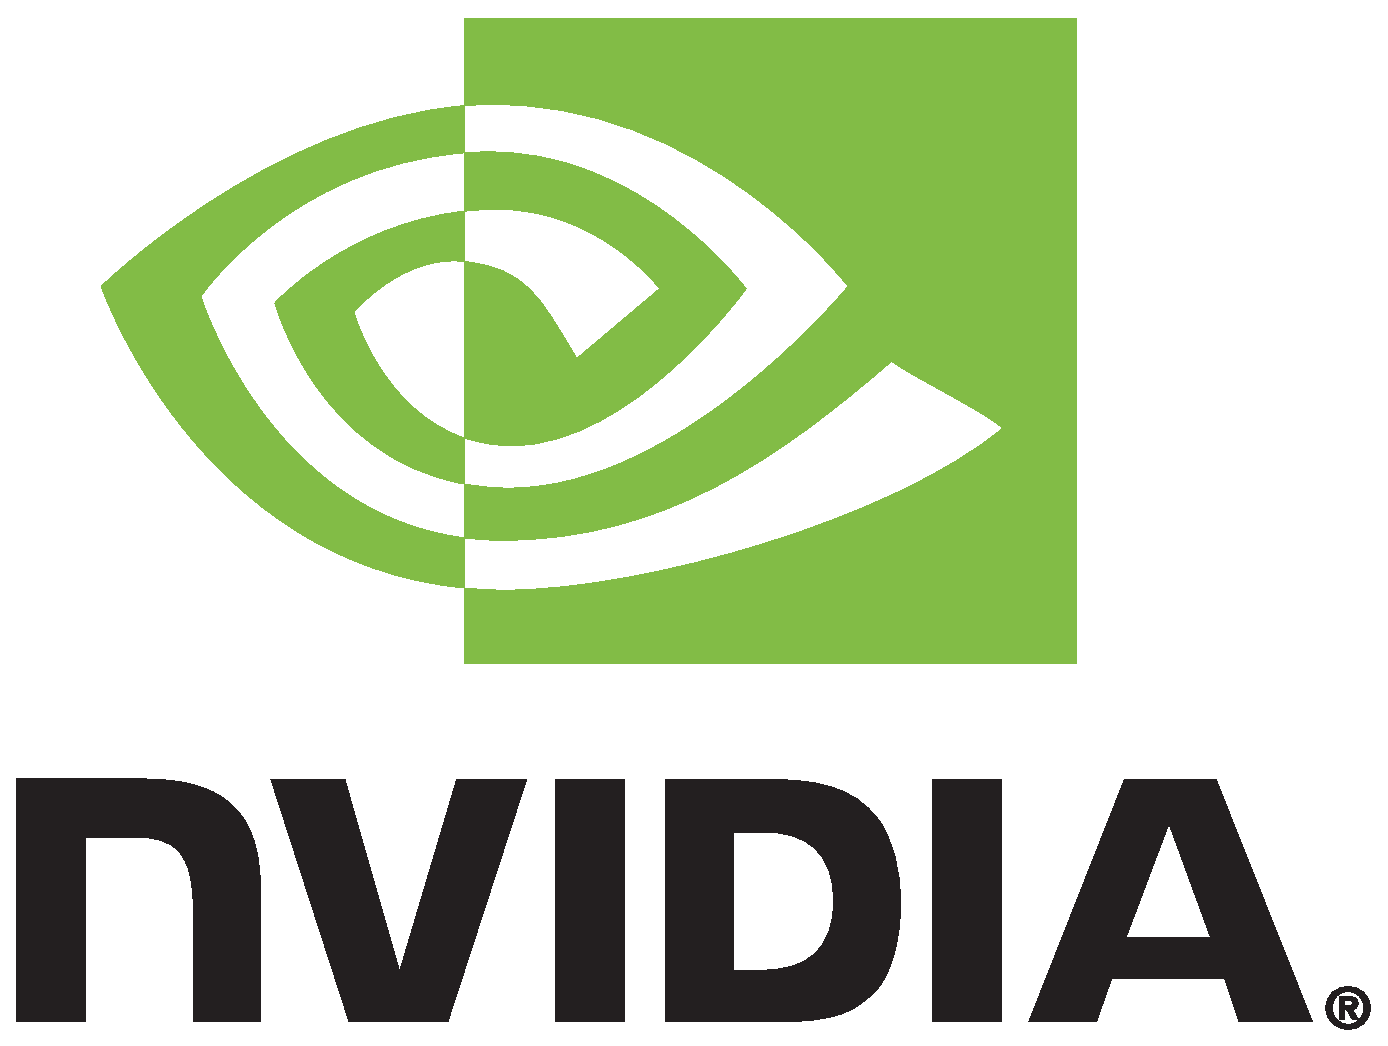
\includegraphics[width=3cm]{../media/logo/NVLogo_2D.eps}
    \vspace{0.75cm}
    \\}
\date{\today}

\begin{document}

\frame{\titlepage}

%\section[Outline]{}
\begin{frame}{Outline}
\tableofcontents
\end{frame}

\addtobeamertemplate{frametitle}{}{%
\begin{textblock*}{200mm}(.75\textwidth,-0.35cm)
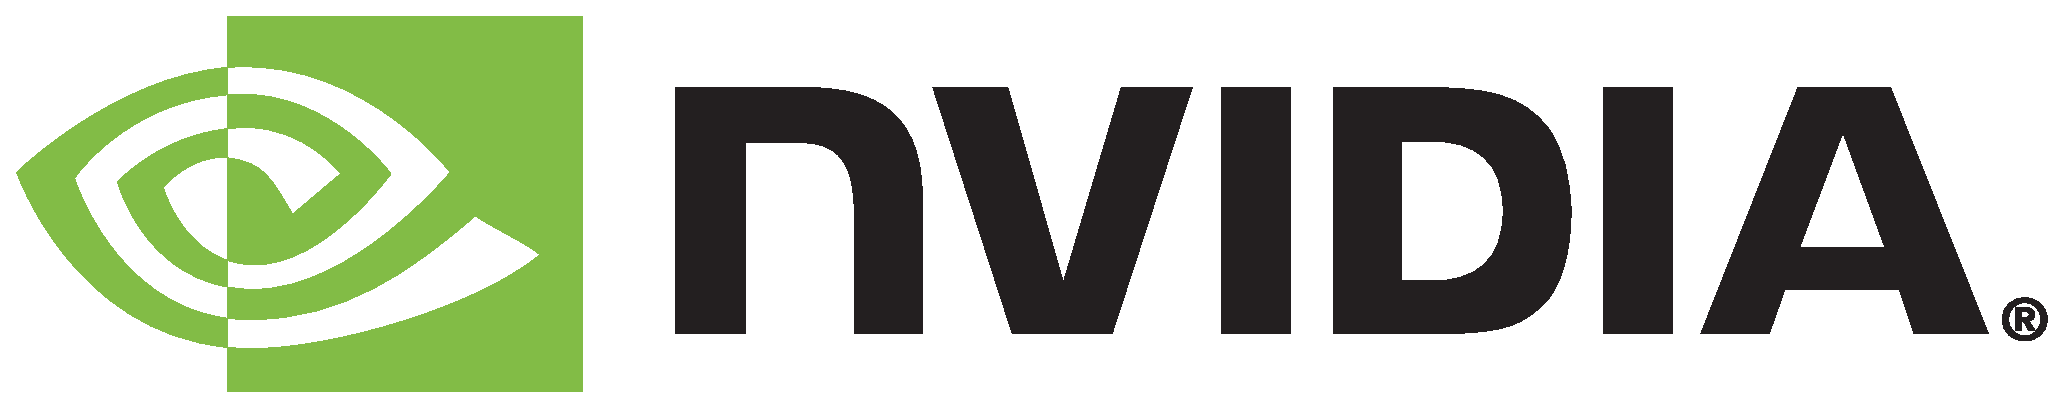
\includegraphics[width=3cm]{../media/logo/NVLogo_2D_H.eps}
\end{textblock*}}

\addtobeamertemplate{navigation symbols}{}{%
    \usebeamerfont{footline}%
    \usebeamercolor[fg]{footline}%
    \hspace{1em}%
    \insertframenumber/\inserttotalframenumber
}

\section{Introduction}
\begin{frame}{Memory Considerations}
There are two primary aspects of memory management when working with accelerators:
\hfill\break
\begin{itemize}
\itemsep1em
    \item<1->Since the GPU is a physically separate device connected to the host via PCI-e bus, the host and device memories have separate address spaces.
    \item<1->As a throughput oriented compute architecture, the GPU device itself provides five distinctly different memory types for use in kernel development and execution.
\end{itemize}
\hfill\break
Many features in each CUDA release are centralized around robustification of the host/device memory interaction while mastery of the various device memory types is both an art and a science essential to every GPU accelerated application.
\end{frame}

\begin{frame}{Address Spaces in CUDA}
\begin{itemize}
\itemsep1em
    \item<1->The physical address spaces for the CPU (host) and GPU (device) are separate.
    \item<1->The CPU cannot read or write device memory on the GPU.
    \item<1->The GPU cannot read or write the host memory on the CPU.
    \item<1->The host application must explicitly copy data to and from the GPU device memory (using runtime API calls) in order to process it (e.g. {\fontfamily{qcr}\selectfont cudaMalloc} and {\fontfamily{qcr}\selectfont cudaMemcpy}).
\end{itemize}
\end{frame}

\begin{frame}{Virtual Addressing: A Lightning Tour}
\begin{itemize}
    \item<1->Physical memory locations are assigned a consecutive number.
    \item<1->The standard unit of measure is the \emph{byte} and so, for example, a memory devices of size 64 kilobytes would have memory locations 0..65535.
    \item<1->The 16-bit values that specify memory locations are known as \emph{addresses} and the process of computing addresses and operating on the corresponding memory locations is collectively known as \emph{addressing}.
    \item<1->Early computers used \emph{physical addressing} whereby CPU instruction operands would reference physical addresses then read and write the corresponding memory locations directly.
    \item<1->As software became more complex and computers running multiple jobs and/or hosting concurrent users grew more common, it became clear that allowing any program to read or write any physical memory location was suboptimal.
\end{itemize}
\end{frame}

\begin{frame}{Virtual Addressing: A Lightning Tour}
\begin{itemize}
\itemsep1em
    \item<1->Modern computers implement \emph{virtual addressing} where each program (process) gets its own virtual address space.
    \item<1->Using virtual addressing, processes specify virtual addresses to be translated into physical addresses by performing a series of lookups into tables setup by the operating system.
    \item<1->In most systems, the virtual address space is divided into \emph{pages} with units of addressing that are at least 4096 bytes in size.
    \item<1->To perform translation, the hardware looks up a \emph{page table entry} (PTE) that specifies the physical address where the page's memory resides.
    \item<1->This address indirection allows a contiguous virtual address space to map to discontiguous pages in physical memory.
    %\item<1->When an application attempts to read or write a memory locations whose page has not been mapped to physical memory, the hardware signals a fault that must be handled by the operating system.
\end{itemize}
\end{frame}

\begin{frame}{Virtual Addressing: A Lightning Tour}
\begin{itemize}
\itemsep1em
    \item<1->When an application attempts to read or write a memory locations whose page either has not been mapped to physical memory yet or has been ejected for inactivity, the hardware signals a fault that must be handled by the operating system.
    \item<1->In practice, at a minimum, the virtual address is segmented into distinct partitions: an index into a ``page directory'' containing many page tables and an index into the page-table specified by the first index.
    \item<1->This type of hierarchical design reduces the amount of memory needed for the page tables and enables inactive page tables to be marked nonresident and swapped to disk, much like inactive pages of memory.
\end{itemize}
\end{frame}

\begin{frame}{Virtual Addressing: A Lightning Tour}
\begin{itemize}
%\itemsep1em
    \item<1->Address translation is performed on \emph{every} memory access performed by the CPU.
    \item<1->To optimize address translation, the CPU contains special hardware caches called translation lookaside buffers (TLBs) and ``page walkers'' that resolve cache misses in the TLBs by reading the page tables.
    \item<1->Today CPUs include hardware support for ``unified address spaces'' where multiple CPUs can access each others memory efficiently.  This hardware mechanism is called Hyper Transport (HT) on AMD chips and QuickPath Interconnect (QPI) on Intel chips.
    \item<1->Since these hardware facilities enable CPUs to access any memory location in the system, this allows reference to ``the CPU'' and ``CPU address space'' irrespective of the number of CPUs in the system.
\end{itemize}
\end{frame}

\begin{frame}{Virtualized Host Memory}
\begin{itemize}
%\itemsep1em
    \item<1->On all operating systems that run CUDA, host memory is \emph{virtualized}.  The operating system component that manages virtual memory is called the \emph{virtual memory manager} or VMM.
    \item<1->Physical pages of memory, usually 4KB or 8KB in size, can be relocated without changing their virtual address.
    \item<1->In particular, these pages can be swapped to disk -- effectively enabling the system to have more virtual memory than physical memory.
    \item<1->When a page is marked ``nonresident'', an attempt to access the page will signal a page fault to the operating system.
    \item<1->The page fault signal prompts the OS to find a physical page avaliable to copy the data from disk and resume execution with the virtual page pointing to the new physical location.
\end{itemize}
\end{frame}

\begin{frame}{Host Memory: Direct Access}
\begin{itemize}
\itemsep1em
    \item<1->The VMM monitors memory activity and uses heuristics to decide when to ``evict'' pages to disk and resolves the pages faults that happen when evicted pages are referenced.
    \item<1->Additionally, the VMM provides services to hardware drivers to facilitate direct access of host memory by the hardware.
    \item<1->Many peripherals such as disk controllers, network controllers, and GPUs  read and/or write host memory using a VMM provided facility known as \emph{direct memory access} (DMA).
    \item<1->DMA enables the hardware to operate concurrently with the CPU.  Whatever the peripheral device, without DMA, the device driver must use the CPU to copy data to or from special hardware buffers.
\end{itemize}
\end{frame}

\begin{frame}{Host Memory: Page-Locking}
\begin{itemize}
\itemsep1em
    \item<1->To facilitate DMA, the VMM provides a service called \emph{page-locking} whereby the VMM marks pages as ineligible for eviction and therefore the physical address can not change.
    \item<1->Once memory is page-locked, drivers can program their DMA hardware to reference the physical addresses of that memory.
    \item<1->Note that page-locking memory makes the underlying physical memory unavailable for other uses by the operating system.
    \item<1->Page-locking a lot of memory can have adverse effects on system performance.
    \item<1->Page-locked memory is sometimes known as \emph{pinned} memory.  The idea is that since the OS can not change the physical address then that memory has been ``pinned in place''.
\end{itemize}
\end{frame}

\begin{frame}{Host Memory: Pinned Memory}
\begin{itemize}
%\itemsep1em
    \item<1->From the OS point of view, the terms \emph{pinned} and \emph{page-locked} are synonymous.
    \item<1->However, from the CUDA point of view, \emph{pinned} memory is page-locked but also tracked by the device driver and mapped for access by the hardware.
    \item<1->In CUDA, pinned memory is allocated and freed using {\fontfamily{qcr}\selectfont cudaHostAlloc()} and {\fontfamily{qcr}\selectfont cudaHostFree()}.  Host memory allocated this way is paged-locked and configured for DMA by the current CUDA context.
    \item<1->The CUDA driver tracks the memory ranges allocated in this way and automatically accelerates memcpy operations that reference pinned memory.
    \item<1->Asynchronous memcpy operations only work with pinned memory.  GPUs cannot access pageable memory at all.
\end{itemize}
\end{frame}

\begin{frame}{Host Memory: Mapped Pinned Memory}
\begin{itemize}
%\itemsep1em
    \item<1->By default, pinned memory is not mapped into the CUDA address space and is not accessible within a CUDA kernel.
    \item<1->Memory that has been both pinned and \emph{mapped} into the address space of the CUDA context allows CUDA kernels to both read and write those memory addresses.
    \item<1->For integrated GPUs, mapped pinned memory enables \href{http://docs.nvidia.com/cuda/cuda-c-best-practices-guide/\#zero-copy}{\color{blue}\emph{zero copy}}: Since the host (CPU) and device (GPU) share the same memory pool, they can exchange data without explicit copies.
    \item<1->On discrete GPUs, mapped pinned memory is advantageous only in certain cases with small amounts of data since the data is not cached on the GPU.
    \item<1->As of CUDA 4.0, if \emph{unified virtual addressing} (UVA) is in effect, all pinned host allocations are mapped.
\end{itemize}
\end{frame}

\begin{frame}{Unified Virtual Addressing}
\begin{itemize}
%\itemsep1em
    \item<1->A feature called \emph{unified virtual addressing} (UVA) was introduced in CUDA 4.0.
    \item<1->When UVA is in force, the CUDA driver allocates memory for both CPUs and GPUs from the same virtual address space.
    \item<1->The CUDA driver accomplishes UVA by having its initialization routine perform large virtual allocations from the CPU address space and then mapping subsequent GPU allocations into those address ranges.  Note that these large initial virtual allocations are not backed by physical memory.
    \item<1->Under UVA, for mapped pinned allocations, the GPU and CPU pointers are the same.  For other types of allocation, the driver can infer the device for which a given allocation was performed from the address.
    \item<1->However, even when UVA is in effect, the CPU(s) cannot access device memory and, by default, the GPU(s) cannot access one another's memory.
\end{itemize}
\end{frame}

\begin{frame}{Notes on Unified Virtual Addressing}
\begin{itemize}
\itemsep1em
    \item<1->UVA is supported on all 64-bit platforms and 64-bit Windows via the \href{http://http.developer.nvidia.com/ParallelNsight/2.1/Documentation/UserGuide/HTML/Content/Tesla_Compute_Cluster.htm}{\color{blue}TCC driver} since the WDDM driver does not yet support UVA.
    \item<1->The TCC driver is available only with enterprise Tesla compute GPUs and can be enabled using the {\fontfamily{qcr}\selectfont nvidia-smi} utility.
    \item<1->Since x64 CPUs support 48-bit virtual address spaces (256 terabytes), while CUDA enabled GPUs only support 40 bit, applications using UVA should make sure CUDA gets initialized early to guard against CPU code using virtual address needed by CUDA.
\end{itemize}
\end{frame}

\begin{frame}{Peer-to-Peer Memory Mapping}
\begin{itemize}
%\itemsep1em
    \item<1->UVA is also a necessary precondition for enabling \href{http://docs.nvidia.com/cuda/cuda-c-programming-guide/index.html\#peer-to-peer-memory-access}{\color{blue}peer-to-peer} (P2P) transfer of data directly across the PCIe bus effectively bypassing host memory.
    \item<1->Because UVA is always in force when using peer-to-peer access, the address ranges for different devices do not overlap, and the driver (and runtime) can infer the owning device from the pointer values.
    \item<1->Peer-to-peer mappings of device memory enable a kernel running on one GPU to read and/or write memory that resides in another GPU.
    \item<1-> Since the GPUs can only ``talk'' at PCI-e rates, GPUs should only exchange modest amounts of data.
    \item<1->However, the advent of \href{http://www.nvidia.com/object/nvlink.html}{\color{blue}NVLINK} allows GPUs to exchange data with much higher bandwidth enabling more diverse peer-to-peer interactions.
\end{itemize}
\end{frame}

\begin{frame}{Peer-to-Peer Memory Mapping}
\begin{itemize}
%\itemsep1em
    \item<1->For P2P addressing to work, the following conditions apply:
    \begin{itemize}
        \item<1->Unified virtual addressing (UVA) must be in effect.
        \item<1->The GPUs must be SM 2.x or higher.
        \item<1->The GPUs must be based on the same chip set
        \item<1->The GPUs must be on the same I/O hub.
    \end{itemize}
    \item<1-> Peer-to-Peer access uses a small amount of extra memory to hold more page tables and makes memory allocation more expensive, since the memory must be mapped for all participating devices.
    \item<1->Note that peer-to-peer mappings are thus not enabled automatically.  P2P must be specifically requested by calling {\fontfamily{qcr}\selectfont cudaDeviceEnablePeerAccess()}.
    \item<1->Once peer-to-peer access has been enabled, all memory in the peer device, including new allocations, is accessible to the current device until {\fontfamily{qcr}\selectfont cudaDeviceDisablePeerAccess()} is called.
\end{itemize}
\end{frame}

\begin{frame}{Unified Managed Memory}
Here we reach the full arc of our journey through the host and device memory interactions within CUDA. Unified Memory represents the forefront of the CUDA programing model and paves the way for exciting features in the upcoming release of \href{https://devblogs.nvidia.com/parallelforall/cuda-8-features-revealed/}{\color{blue}CUDA 8}.

\begin{itemize}
    \item<1->\href{http://docs.nvidia.com/cuda/cuda-c-programming-guide/index.html\#um-unified-memory-programming-hd}{\color{blue}\emph{Unified Memory}} was introduced in CUDA 6.0 with the intent to simplified memory management by automatically migrating the necessary data back and forth between host and device -- eliminating explicit memcpy calls and  \href{https://devblogs.nvidia.com/parallelforall/unified-memory-in-cuda-6/}{\color{blue}deep copy} issues.
    \item<1->In a nutshell, the driver automatically migrates data between GPU and CPU, so that it looks like CPU memory to code running on the CPU, and like GPU memory to code running on the GPU.
    \item<1->Unified memory is effectively all the programatic benefits of UVA zero-copy but scalable since the driver will automatically migrate the necessary data, at the level of individual pages, between host and device memory.
\end{itemize}
\end{frame}

\begin{frame}[fragile]{Unified Managed Memory}
\begin{itemize}
    \item<1->The term \emph{managed memory} refers to memory allocated dynamically on the host via {\fontfamily{qcr}\selectfont cudaMallocManaged()} or statically declared in global scope using the {\fontfamily{qcr}\selectfont \_\_managed\_\_} annotation:
    \end{itemize}
\begin{lstlisting}[]
  __device__ __managed__ int y[N];
\end{lstlisting}

\begin{itemize}
    \item<1->It is very important to keep in mind that managed memory is visible to all available devices in the system.  To constrain which devices are visible/exposed to the application, set the environment variable \href{http://docs.nvidia.com/cuda/cuda-c-programming-guide/index.html\#env-vars}{\color{blue}{\fontfamily{qcr}\selectfont CUDA\_VISIBLE\_DEVICES}}.
    \item<1->Managed memory is \emph{interoperable} with un-managed device-specific memory allocations such as {\fontfamily{qcr}\selectfont cudaMalloc()}.  A kernel can utilize both managed and un-managed memory.
\end{itemize}
\end{frame}

\begin{frame}{Unified Managed Memory: Coherence}
\begin{itemize}
    \item<1->Unified Memory attempts to optimize memory performance by migrating data towards the device where it is being accessed.
    \item<1->The physical location of data is invisible to the program and may be changed at any time, but accesses to the virtual address of the data will remain valid and coherent from any processor regardless of locality.
    \item<1->Note that maintaining coherence is the primary requirement ahead of performance.  Within the constraints of the host operating system, the unified memory management system can either fail accesses or move data in order to maintain global coherence between processors.
    \item<1->The memory system will try to place data in a location where it can most efficiently be accessed without violating coherency.
\end{itemize}
\end{frame}

\begin{frame}{Unified Memory: Exclusive Access}
\begin{itemize}
    \item<1->To help ensure coherency, the Unified Memory programming model puts constraints on data accesses while both the CPU and GPU are executing concurrently.
    \item<1->The device has exclusive access to all managed data while any kernel operation is executing, regardless of whether the specific kernel is actively using the data.
    \item<1->Concurrent host/device accesses, even to different managed memory allocations, will cause a segmentation fault because the page is considered inaccessible to the host.
    \item<1->The behavior of dynamically allocating memory, with {\fontfamily{qcr}\selectfont cudaMallocManaged()} or {\fontfamily{qcr}\selectfont cuMemAllocManaged()}, while the device is active is unspecified until additional work is launched or the device is synchronized.  Attempting to access that memory on the host during this time may or may not cause a segmentation fault.
\end{itemize}
\end{frame}

\begin{frame}{Unified Memory: Exclusive Access}
\begin{itemize}
    \item<1->To help ensure coherency, the Unified Memory programming model puts constraints on data accesses while both the CPU and GPU are executing concurrently.
    \item<1->The device has exclusive access to all managed data while any kernel operation is executing, regardless of whether the specific kernel is actively using the data.
    \item<1->Concurrent host/device accesses, even to different managed memory allocations, will cause a segmentation fault because the page is considered inaccessible to the host.
    \item<1->The behavior of dynamically allocating memory, with {\fontfamily{qcr}\selectfont cudaMallocManaged()} or {\fontfamily{qcr}\selectfont cuMemAllocManaged()}, while the device is active is unspecified until additional work is launched or the device is synchronized.  Attempting to access that memory on the host during this time may or may not cause a segmentation fault.
\end{itemize}
\end{frame}

\begin{frame}{Unified Managed Memory: Multi-GPU}
\begin{itemize}
    \item<1->Managed allocations are automatically visible to all GPUs in a system via the peer-to-peer capabilities.
    \item<1->While multi-GPU systems are able to use managed memory, data does not migrate (i.e. get copied) between GPUs.
    \item<1->Managed memory allocation behaves similarly to unmanaged memory allocations whereby the current active device is the home for the physical allocation and all other GPUs receive peer mappings to the memory (i.e. it's just UVA zero-copy between two devices over PCI-e).
    \item<1->If peer mappings are not available, perhaps due to GPUs of different architectures, then the system will fall back to using zero-copy \emph{host} memory in order to guarantee data visibility.  That is, \textbf{double} zero-copy $GPU(i) \rightarrow host \rightarrow GPU(j)$ over PCI-e (don't do this).  More details in the \href{http://docs.nvidia.com/cuda/cuda-c-programming-guide/index.html\#um-managed-memory}{\color{blue}docs}.
\end{itemize}
\end{frame}

\begin{frame}{Unified Managed Memory: Profiling}
\begin{itemize}
    \item<1->Both {\fontfamily{qcr}\selectfont \textbf{nvprof}} and {\fontfamily{qcr}\selectfont \textbf{nvvp}} have been updated to provide detailed Unified Memory profiling capabilities.
    \item<1->Use {\fontfamily{qcr}\selectfont \textbf{nvprof} --profile-api-trace runtime} to get details on runtime-api calls for managed memory
    \item<1->Use {\fontfamily{qcr}\selectfont \textbf{nvprof} --print-gpu-trace} to print individual kernel invocations (including CUDA memcpy's/memset's)
                        and sort them in chronological order.  In particular, looking for Unified Memory Memcpy HtoD and DtoH.
    \item<1->Use {\fontfamily{qcr}\selectfont \textbf{nvprof} --unified-memory-profiling off} to disable unified memory profiling 
    \item<1->Launch {\fontfamily{qcr}\selectfont \textbf{nvvp}}, Create New Session, and be sure to check the option for ``Enable unified memory profiling''.
    \item<1->When viewing the execution profile in {\fontfamily{qcr}\selectfont \textbf{nvvp}}, be sure to use the ``zoom in'' feature to get better view of the action.

\end{itemize}
\end{frame}

\begin{frame}{Multi-GPU Applications: NCCL}
\begin{itemize}
    \item<1->The Unified Memory system has many benefits for CUDA programers and their applications but multi-GPU programing doesn't exactly standout in this regard.
    \item<1->Today it is not uncommon for servers to contain 8 or more GPU devices. In principle, scaling an application from one to many GPUs should provide a significant performance boost. In practice, the benefits of multi-GPU development can be difficult to obtain -- typically for three (correlated) reasons:
    \begin{itemize}
        \item<1->Poor exposure of parallelism in the problem
        \item<1->Devices exchange too much data and spend more time communicating than computing
        \item<1->PCI-e bandwidth limitations
    \end{itemize}
    \item<1->\href{https://devblogs.nvidia.com/parallelforall/fast-multi-gpu-collectives-nccl/}{\color{blue}NCCL} (pronounced ``Nickel'') is an open-source library from NVIDIA containing multi-GPU collective communication primitives in the spirit of MPI that are topology-aware and can be ``easily'' integrated into CUDA applications.
    \item<1->NCCL with \href{http://www.nvidia.com/object/nvlink.html}{\color{blue}NVLINK} creates a truly unique multi-GPU development opportunity.
\end{itemize}
\end{frame}

\begin{frame}[fragile]{The Future of Unified Memory}
\begin{itemize}
	\item<1->On Kepler and Maxwell architectures, bulk managed data migration to the device is triggered by a kernel launch.
	\item<1->Pages of device memory are allocated \textbf{before} they are used.  This means it is not possible to oversubscribe device memory.
\end{itemize}
\begin{lstlisting}[caption={Fails on Kepler and Maxwell}]
  void foo() {
  
    // init pointer to data
    char *data;
  
    // specify 32 GB of memory in bytes
    size_t numBytes = 32*1024*1024*1024; 
  
    // Allocate 32 GB
    cudaMallocManaged(&data, numBytes);
  }
\end{lstlisting}
\end{frame}

\begin{frame}[fragile]{The Future: GPU Page Faults}
\begin{itemize}
	\item<1->On new Pascal architecture, managed memory uses GPU page faults rathe than bulk data migration.  Pages of device memory are populated and data migrated on first touch.
	\item<1->When kernel launches and accesses memory, if device does not have a VA translation, it issues an interrupt to CPU.
	\item<1->The Unified Memory driver could decide to map the associated memory or migrate depending on various heuristics.
	\item<1->With Pascal \emph{on-demand paging} it is possible to allocate much more memory than is physically available on the device.
	\item<1->Furthermore, the Pascal architecture provides more support for concurrent access to memory from CPU and GPU (page-level coherency).  
	\item<1->As an example, with very large graph processing, it can be difficult to predict which edges and vertices will need to be resident on the device.   With Pascal, bring only necessary vertices/edges on-demand allowing work on very large graphs that cannot fit into GPU memory.
\end{itemize}
\end{frame}

\begin{frame}[fragile]{The Future: Unified Memory Hints}
\begin{itemize}
	\item<1->In general want to minimize GPU page faulting. Fault handling can take 10s of $\mu$s while execution stalls.
	\item<1->Clearly, want to keep data local to the accessing processor to minimize latency and maximize bandwidth.  However, it is not difficult to think of situations which could induce ``thrashing'' whereby the data migration overhead exceeds locality benefits.
	\item<1->The CUDA 8.0 runtime API will include unified memory ``hints'' such as {\fontfamily{qcr}\selectfont cudaMemPrefetchAsync} and {\fontfamily{qcr}\selectfont cudaMemAdvise} which allow for specification of allocation and usage policies for memory regions and manual prefetching.
	\item<1->For example, using {\fontfamily{qcr}\selectfont cudaMemPrefetchAsync} can prefetch large array of data to avoid excessive number of expensive page faults on kernel launch.
	\end{itemize}
\end{frame}

\begin{frame}
\begin{center}Source Code Examples\end{center}
\end{frame}

%\begin{frame}[fragile]{CUDA Malloc/Memcpy Example}
%\lstinputlisting[language=C++,firstline=10,lastline=29,caption={Initializing memory on the device}]{../src/vecAdd.cu}
%\end{frame}

\begin{frame}[fragile]{CUDA Malloc/Memcpy Example}
\begin{lstlisting}[caption={The classic CUDA memory initialization strategy.}]
    // number of bytes to alloc for arrays
    size_t numBytes = N*sizeof(float);

    // init host and device pointers
    float *ha, *da;

    // alloc host memory/arrays (pagable memory)
    ha = (float*)malloc(numBytes);

    // mem alloc arrays on the GPU device
    cudaMalloc(&da,numBytes);

    // copy host array to device array (synchronous)
    cudaMemcpy(da, ha, numBytes, cudaMemcpyHostToDevice);

    // launch kernels etc ... (asynchronous)

    // now copy device array to host array (snychronous)
    cudaMemcpy(ha, da, numBytes, cudaMemcpyDeviceToHost);

    // dealloc on host and device
    free(ha);  cudaFree(da);

\end{lstlisting}
\end{frame}

\begin{frame}[fragile]{CUDA Zero-Copy Example}
\begin{lstlisting}[caption={Using cudaHostAlloc allows CUDA kernels to read and write those memory addresses.  Note that kernel launch must reference device pointer.  Only use zero-copy strategy with small amounts of data since the data is not cached on the GPU.}]
    size_t numBytes = N*sizeof(float);

    // init host and device pointers
    float *ha, *da;

    // alloc host memory (host pinned, device mapped)
    cudaHostAlloc(&ha,numBytes,cudaHostAllocMapped);

    // get device pointers for mapped memory
    cudaHostGetDevicePointer(&da, ha,0);

    // launch kernels etc ...
    mykernel<<<blksz, grdsz>>>(da);

    // wait for kernel to finish
    cudaDeviceSynchronize();

    // free host pointers
    cudaFreeHost(ha);
\end{lstlisting}
\end{frame}

\begin{frame}[fragile]{CUDA Zero-Copy with UVA Example}
\begin{lstlisting}[caption={Using cudaHostAlloc allows CUDA kernels to read and write host memory addresses.  With UVA in effect (introduced in CUDA 4.0), host pointers can be directly passed to kernel launch.  Again, only use zero-copy strategy with small amounts of data since the data is not cached on the GPU.}]
    // number of bytes to alloc for arrays
    size_t numBytes = N*sizeof(float);

    // init host pointer
    float *ha;

    // alloc host memory (host pinned, device mapped)
    cudaHostAlloc(&ha,numBytes,cudaHostAllocMapped);

    // launch kernels etc ...
    mykernel<<<blksz, grdsz>>>(ha);

    // wait for kernel to finish
    cudaDeviceSynchronize();

    // free host pointers
    cudaFreeHost(ha);
\end{lstlisting}
\end{frame}

\begin{frame}[fragile]{CUDA Managed Memory Example}
\begin{lstlisting}[caption={Using cudaMallocManaged (introduced in CUDA 6.0) eliminates all explicit memory copies.  Thanks to UVA, host pointers can be passed directly to kernal launch.  Unlike zero-copy,  using managed memory is generally quite scalable since the driver will automatically migrate the necessary data back and forth between host and device.}]
    // number of bytes to alloc for arrays
    size_t numBytes = N*sizeof(float);

    // init host pointer
    float *ha;

    // alloc fully managed host memory
    cudaMallocManaged(&ha,numBytes);

    // launch kernels etc ...
    mykernel<<<blksz, grdsz>>>(ha);

    // wait for kernel to finish
    cudaDeviceSynchronize();

    // free host pointers
    cudaFreeHost(ha);
\end{lstlisting}
\end{frame}

\begin{frame}[fragile]{Unified Memory: Exclusive Access}
\begin{lstlisting}[caption={Do not do this.  The device has exclusive access to managed memory while kernel launch is active, regardless of whether the kernel references the memory accessed by the host.}]

  // static allocation of manage memory in global scope
  __device__ __managed__ int x, y=2;

  // define generic kernel
  __global__ void kernel() { x = 10; }

  int main(void) {

      // launch kernel (asynchronous)
      kernel<<<1,1>>>();

      // access managed memory while kernel executing ...
      y = 20; // ERROR -- GPU has exclusive access

      // wait for kernel to finish
      cudaDeviceSynchronize();

      return 0;
}
\end{lstlisting}
\end{frame}

\begin{frame}[fragile]{GPUDirect P2P UVA Memory Example}
\begin{lstlisting}[caption={Exchanging memory between peer devices with UVA in effect.  What makes P2P exchange special is that devices exchange data directly, effectively bypassing the host.  This feature is often referred to as ``GPUDirect P2P Transfer''.  Without P2P capabilities enabled there is an extra copy involved over PCI-e as data from the source device must be copied to the host and then copied again from the host to the destination.} ]
  // check if each device can support peer access
  cudaDeviceCanAccessPeer(&peerAccess01, 0, 1);
  cudaDeviceCanAccessPeer(&peerAccess10, 1, 0);

  // enable peer access: device 0 to device 1
  cudaSetDevice(0);  
  cudaDeviceEnablePeerAccess(1,cudaPeerAccessDefault);
  
  // enable peer access: device 1 to device 0
  cudaSetDevice(1);  
  cudaDeviceEnablePeerAccess(0,cudaPeerAccessDefault);

  // UVA enabled copy, memcpy knows who owns the pointers
  cudaMemcpy(buf0, buf1, numBytes, cudaMemcpyDefault);
\end{lstlisting}
\end{frame}

\end{document}